\documentclass[convert={density=300,size=1080x800,outext=.png}]{standalone}

\usepackage[latin1]{inputenc}
\usepackage{tikz}

\usetikzlibrary{shapes,arrows,calc,fit,positioning}

\begin{document}
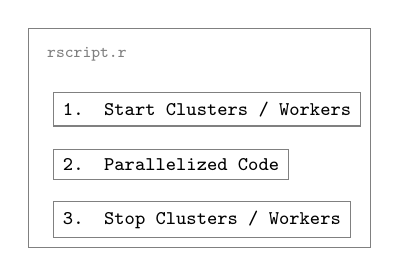
\begin{tikzpicture}[
  node distance=7mm,
  title/.style={font=\fontsize{6}{6}\color{black!50}\ttfamily},
  typetag/.style={rectangle, draw=black!50, font=\scriptsize\ttfamily, anchor=west}
]
  \node (decomp) [title] { rscript.r };

  \node (di) [below=of decomp.west, typetag, xshift=2mm] { 1. Start Clusters / Workers };
  \node (dr) [below=of di.west, typetag] { 2. Parallelized Code };
  \node (dnc) [below=of dr.west, typetag] { 3. Stop Clusters / Workers };

  \node [draw=black!50, fit={(decomp) (di) (dr) (dnc)}] {};
\end{tikzpicture}

\end{document}